\section{Study Settings}

%\kn{This paragraph requires a motivation. The details of Boa's study must be described upfront. Something like "Boa et al.'s study performs ..... Since their study also involved a static analysis component whose impact was not measured, we perform a non-exact replication to understand the impact static analysis may have had in the results...}


In this section
we present the settings of our study, whose goal is to build a general understanding of the implications of using static analysis algorithms
to complement a dynamic analysis approach
for mining Android sandboxes. % We also investigate how static analysis can improve the performance of mining sandboxes, in the task of identifying malicious behavior.
To achieve this goal, we answer the following research questions.

\begin{enumerate}[(RQ1)]
 
 \item What is the impact of the DroidFax static analysis algorithms into the results of the \blls?
  
 \item What is the effective performance of each test generation tool, in terms of the number of detected malware, when we
   discard the contributions of the DroidFax static analysis algorithms?

 \item What are the benefits of using taint
 analysis algorithms to complement the dynamic analysis approach for mining sandboxes?
\end{enumerate}

%\kn{Droidfax comes out of nowhere. We should introduce this or if already introduced earlier, remind the readers of where it stands with the Bao study in the first line of this section when describing boas study}

Answering the research questions RQ1 and RQ2 allows us to expose a possible overestimation in terms of the number of detected malware by each sandbox, constructed by the test
generation tools explored in \blls. Ignoring the implications of DroidFax in the \blls might have introduced a possible threat to their conclusions. Answering the third research question
allows us to open up the possibility of finding new strategies for designing mining sandbox techniques, complementing the performance of
dynamic analysis through the use of static analysis algorithms.
We conducted two studies to answer the research questions above. In the
first study we leverage DroidXP~\cite{DBLP:conf/scam/CostaMCMVBC20} (Section~\ref{sec:droidxp}) to replicate
the \blls. We present the settings of this first study in Section~\ref{sec:set1}.
In the second study we use
FlowDroid~\cite{DBLP:conf/pldi/ArztRFBBKTOM14} to investigate the 
suitability of taint analysis algorithms for mining Android sandboxes.
We present the settings of the second study in Section~\ref{sec:set2}. 


\subsection{The DroidXP benchmark}\label{sec:droidxp}

We used DroidXP to systematically assess and compare the performance of test generation tools for mining android sandboxes. DroidXP relies on a
simple \emph{Command Line Interface} (CLI) that simplifies the integration of different test generation tools and favors the setup and execution 
of the experiments. DroidXP also relies on DroidFax, which instruments Android apps and collects relevant information about
their execution, including the set of sensitive APIs a given
app calls during a test execution. DroidFax also collects inter-component communication (ICC) using  static
program analysis.


The DroidXP CLI provides commands for listing all test case
generation tools (executing the project with the option ``list-tools'') that had been
integrated into the benchmark and commands that execute the experiments. An
experiment run can be configured according to several parameters, including:

\begin{itemize}
    \item \texttt{-tools}: Specifies the test tools used in the experiment
    \item \texttt{-t}: Specifies the threshold (in seconds) for the execution time in the experiment
    \item \texttt{-r}: Specifies the number of repetitions used in the experiment
    \item \texttt{-output-format}: Specifies the output format
    \item \texttt{--debug}: Specifies to run in DEBUG mode (default: false)
    \item \texttt{--disable-static-analysis}: Disable DroidFax static analysis phase (default: false)
\end{itemize}

Figure~\ref{fig:benchArq} shows the DroidXP architecture, based on the pipes-and-filters architectural style \cite{architecture-book}. 
The architecture includes three main components; where each component is responsible for a specific phase of the
benchmark (instrumentation, execution, and result analysis).

\begin{figure*}[thb]
  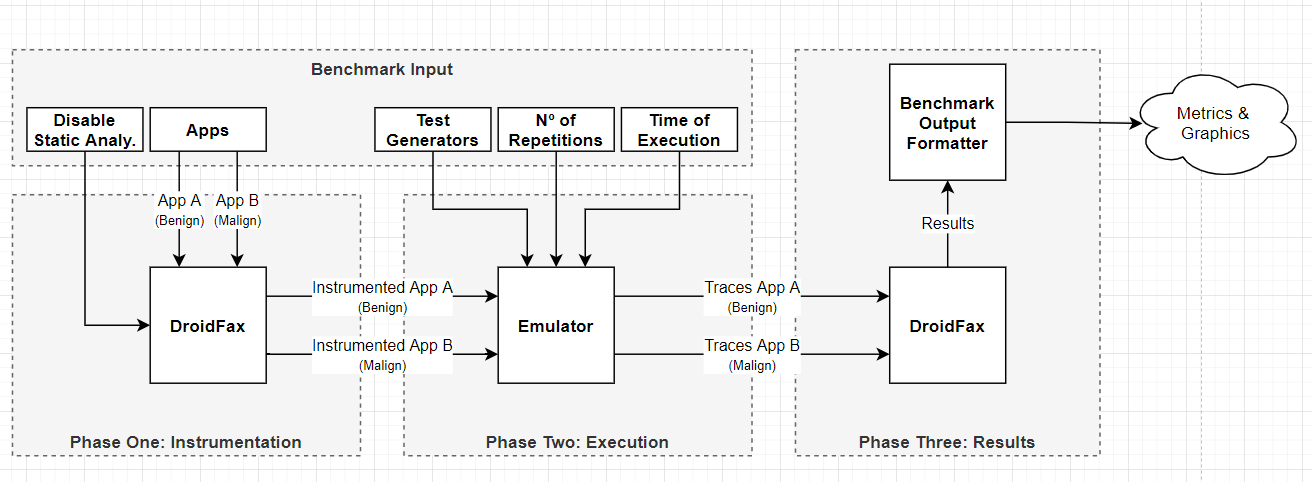
\includegraphics[width=1\textwidth]{images/benchmark4.png}
  \label{benchArq}
  \caption{Benchmark architecture}
  \label{fig:benchArq}
\end{figure*}
\subsubsection{Phase 1: Instrumentation}

In the first phase, a researcher must define the corpus of APK files DroidXP should consider during a benchmark execution. After that, DroidXP starts the DroidFax service that instruments each APK file, so that DroidXP would be able to collect data about each execution. To improve the performance of the benchmark, the instrumentation phase runs only once for each APK. In this phase, the DroidFax tool also runs some static analysis procedures---when the option \texttt{--disable-static-analysis} is not set.

\subsubsection{Phase 2: Execution}

In this phase, DroidXP installs an (already instrumented) APK file into
an Android emulator, and then executes a test case generation tool
during a period of time. This process repeats for every test case generation
tool and APK files. To provide repeatability of the experiment, DroidXP removes all data stored in the emulator before starting
a new execution. That is, every execution uses a \emph{fresh} emulator,
without any information that might have been kept during
previous executions. 

It is relatively easy to add new test
case generation tools into DroidXP. To achieve this goal, it leverages the Strategy Design
pattern~\cite{patterns-book}, which sets a contract between a family of classes that, in our case, abstracts the particularities
for running each tool we want to integrate into DroidXP.
%To carry out our replication study, we successfully integrated all
%test generation tools previously mentioned into DroidXP: Monkey, DroidBot, DroidMate, and
%Humanoid. 

\subsubsection{Phase 3: Result Analysis}

During the execution of the instrumented apps, all data that is relevant to our
research is collected by Logcat~\cite{Logcat}, one of the Android SDK's native tools. Logcat dumps a log from the Android emulator
while the already instrumented app is in execution. The part of the log we analyze in this phase comprises
the data sent by the methods within the Android app that were instrumented on the first
phase using the DroidFax tool. 

This data includes method coverage from the execution of each test generator tool and the
set of sensitive APIs the app calls during its execution. This set of calls to
sensitive APIs is necessary to estimate the test generator performance in identifying malicious apps---by spotting
differences between the sensitive API accessed by each version of an app (benign or malign).
In the end, the benchmark outputs the results of the experiment, which gives the
performance of one or more testing generator tools in mining sandboxes.

We used the DroidXP infrastructure to conduct the replication of
the \blls, whose settings we present in the following section. 

\subsection{First Study: A replication of the \blls}\label{sec:set1}

The \blls reports the results of an empirical study that compares the performance of test generation tools to mine Android
sandboxes, based on the calls to sensitive APIs from 102 pairs (benign / malign) of Android apps. In their work, \emph{performance} is
measured as the total number of malwares a sandbox is able to identify when comparing the calls to sensitive APIs made by
the benign and malign versions of the app. A \emph{hit} occurs whenever a sandbox finds that the malicious version of an app calls
additional sensitive APIs, in comparison to the calls from the corresponding benign version.
Nonetheless, the \blls uses DroidFax to instrument the Android apps, even though DroidFax also
collects calls to sensitive APIs using static analysis algorithms. Since the \blls does not
compute the possible impact of DroidFax into the performance of the test generation tools,
here we replicate their work to understand the impact of the DroidFax static analysis algorithms into the \blls results.

Our replication differs from the original work in a few decisions. First, here we isolate
the effect of the DroidFax static analysis algorithms, in the task to identify malicious apps. In addition, although we use the same dataset of
$102$ pairs of Android apps used in the \blls, here we discarded $6$ pairs for which
we were not able to instrument---out of the $102$ pairs used in the original work. We also introduced a recent test generator tool (Humanoid ~\cite{DBLP:conf/kbse/LiY0C19}), which
has not been considered in the previous work. Finally, we extended the execution time of each test generation tool,
executing each app from the test generation tool for three minutes (instead of one minute in the
original work),
and built the sandboxes after executing each test generation tool
three times---the original work executed each test generation tool
only once. That is, our goal here is not to conduct an
exact replication of the \blls, but instead understand
the role of the DroidFax static analysis algorithms in the
performance of test case generation tools for mining sandboxes.
% The original study executed each app at each tool, for just one minute, and just one time.

Besides Humanoid, our study considers three test generation tools used in the \blls: DroidBot~\cite{DBLP:conf/icse/LiYGC17},
DroidMate~\cite{DBLP:conf/icse/JamrozikZ16}, and Monkey~\cite{Monkey}. We selected DroidBot and DroiMate because they achieved
the best performance on detecting malicious behavior---when considering the $102$ pairs of Android apps (B/M) in the \blls.
It is important to note that here we used a new version of DroidMate (DroidMate-2), since it presents several enhancements
in comparison to the previous version. We also considered the Google's Monkey open source tool, mostly because it is the most
widely used test generation tool for Android~\cite{DBLP:conf/sigsoft/ZengLZXDLYX16}. Monkey is part of the Android SDK
and does not require any additional installation effort. We included Humanoid in our study
because it emulates realistic users, creating human-like test inputs using deep learning techniques.



% In the first study we executed the DroidXP benchmark with its
% default configuration, that is, enabling the DroidFax
% static analysis algorithms and the test generation tools.

We first run the experiment using the default
settings of DroidXP, to explore the four test case generation tools described earlier and a fake test
case generation tool (named \joke). \joke simulates a test tool that does not execute
the Android apps during a benchmark execution. Using this tool, the results
of the dynamic analysis are not considered and we can compute the results with
only the static analysis component of DroidFax (RQ1). Our study executed each pair of
Android app (B/M) in each one of the five test generation tools, including \joke,
for three minutes, and for three times. We then investigate the performance of each tool to detect malicious behaviors in the sandbox
modeled by the test generation tool
under analysis. 


After that, we replicated the analysis using a configuration of DroidXP that disables the DroidFax static analysis algorithm.
Using this new configuration, we executed the benchmark again, using the same dataset of Android apps, the same execution time,
and the same test case generation tools.
The results of this replication allow us to compute the effective performance
of the dynamic analysis tools (RQ2)---that is, ignoring the influence of the
DroidFax static analysis algorithms.
Figure \ref{fig:setup} shows all the phases of our experiments, that explore all sensitive
resources access by both apps (B/M), and the optional configuration DroidXP, that disables DroidFax static analysis.


\begin{figure}[ht]
  \centering{
   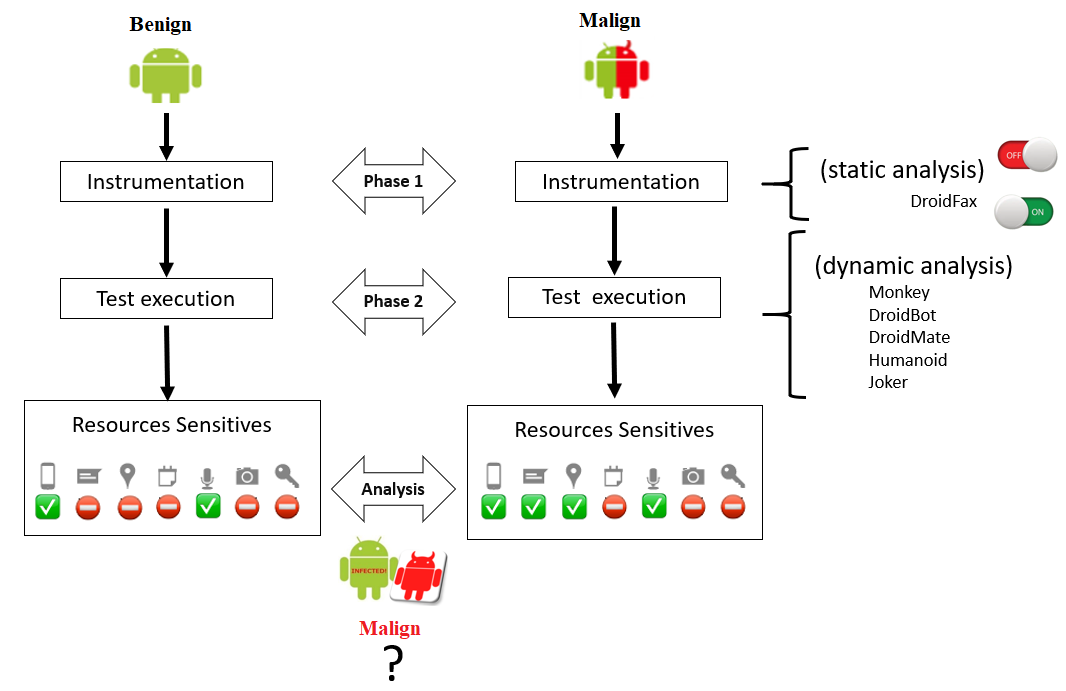
\includegraphics[width=0.75\textwidth]{images/setup3.png}}
   \label{Experiment setup}
   \caption{Experiment setup}
   \label{fig:setup}
 \end{figure}

\subsection{Second Study: Use of Taint Analysis Algorithms for Mining Sandboxes}\label{sec:set2}

In the second study 
we investigate whether or not a more advanced static analysis approach is promising for
mining Android sandboxes. To this end, we leverage the FlowDroid
taint analysis algorithms for Android apps, in order to identify paths between
\emph{sources} and \emph{sinks}. In this case,
our goal is to investigate if it is possible to detect malicious
behavior by comparing the source-sink paths that FlowDroid finds in the
benign / malign versions of the Android apps.

Concerning this second study, a \emph{hit} occurs whenever
FlowDroid finds an additional source-sink path in the malicious version of an app.
Our goal is to answer our third research question using this approach. We use two metrics in this second study:
the total number of malicious apps FlowDroid is able to find and the
execution time for running the taint analysis algorithm for each app.
In this second study we use the same dataset of $96$ pairs of Android apps (B/M),
originally shared in the AndroZoo repository~\cite{DBLP:conf/msr/AllixBKT16} and
also used in the \blls. 


We conduct this investigation in three steps. First, we use
FlowDroid to mine all sources and sinks paths from each benign app, and then enumerate all possible data flows between sources
and sinks. Next, we repeat the the analysis considering the malicious version
of the apps. Finally, we compare the sets of source-sink paths between the benign and malicious
version of an app, in order to reveal the existence of additional paths in the
malicious version. 







